\chapter{\textit{Generalized Partial Global Planning}}\label{sec:gpgp}

O padrão \textit{Generalized Partial Global Planning} (GPGP) atua na coordenação de tarefas locais de cada agente considerando objetivos locais e não locais \cite{decker1992generalizing}. 

%Baseia-se na detecção de relacionamentos nas estruturas de objetivos computacionais dos agentes distribuídos. 

\begin{description}
  \item[Nome do padrão:]  \textit{Generalized Partial Global Planning} (GPGP) ou Planejamento Global Parcial Generalizado.
    \item[Referências:]    \citeonline{de2009introduction}, \citeonline{decker1992generalizing}.
    \item[Categoria:] \textit{Team Structure}.
    \item[Problema:] é adotado para possibilitar a coordenação distribuída; que pode ser descrita como o agendamento das atividades locais de cada agente considerando preocupações e restrições não locais \cite{decker1992generalizing}.
    \item[Solução:] Para abordar o padrão GPGP, será primeiramente apresentada a estrutura PGP exemplificada pela Figura \ref{fig:pgp_agent_level}. O \textit{Agent 1} possui o objetivo global de completar a tarefa \textit{A1}, e duas sub-tarefas concorrentes, \textit{B1} e \textit{C1}. O \textit{Agent 2} possui o objetivo de completar a tarefa \textit{A2}, e duas sub-tarefas \textit{B2} e \textit{D2} \cite{decker1992generalizing}. 
    
    
\begin{figure}[h!]
    \centering
    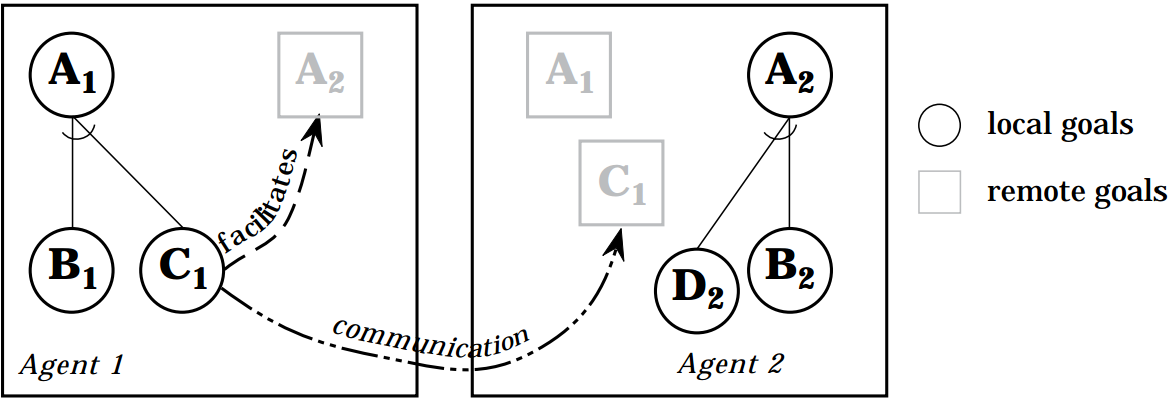
\includegraphics[scale=0.3]{figuras/pgp/pgp_agent_level.png}
    \caption{Exemplo de estrutura PGP. Fonte: \citeonline{decker1992generalizing}.}
    \label{fig:pgp_agent_level}
\end{figure}

    No algoritmo PGP, os agentes \textit{Agent 1} e \textit{Agent 2} vão trocar seus objetivos de mais alto nível, chamados \textit{System Goals}.
    Havendo ciência desta informação, o \textit{Agent 1} pode determinar que sua sub-tarefa local C1 facilita a tarefa A2  \cite{decker1992generalizing}. 
    
    Isto indica que a tarefa C1, de algum modo, é útil para que se complete A2.
    Informações sobre o status da sub-tarefa C1 são enviadas ao \textit{Agent 2} permitindo-o rearranjar sua programação para lidar com informações futuras. Similarmente, o fato de C1 ser uma tarefa facilitadora, torna-a preferível. Por exemplo, se o \textit{Agent 1} possuir duas tarefas concorrentes, sendo uma delas \textit{C1}, e não havendo outra razão para dar preferência à outra, o algoritmo PGP agendará \textit{C1} para ocorrer primeiro  \cite{decker1992generalizing}.
   

A estrutura do PGP não foi projetada apenas para permitir a comunicação de informações necessárias para o planejamento global, mas também para o projeto e análise de algoritmos de coordenação para agentes que operam em ambientes com características diferentes daquelas para as quais o PGP foi projetado . Por exemplo, podem haver agentes heterogêneos - que podem ter diferentes critérios locais de solução de problemas -, agentes dinâmicos - que possuem várias estratégias e métodos diferentes disponíveis para a realização de metas e um conjunto de compensações entre eles - e em tempo real - agentes que podem ter prazos rígidos ou flexíveis \cite{decker1992generalizing}.%

%O GPGP também suporta (mas não prescreve) negociações explícitas entre os agentes e permite que os agentes se comuniquem em diferentes níveis de detalhes. As estruturas de meta construídas, mantidas e comunicadas pelo mecanismo PGP original são incluídas neste modelo.

O Planejamento Global Parcial (PGP) é uma abordagem flexível à coordenação distribuída que permite aos agentes responder dinamicamente à sua situação atual. O GPGP tenta estender a abordagem PGP comunicando informações mais abstratas e organizadas hierarquicamente, detectando de maneira geral as relações de coordenação necessárias aos mecanismos de planejamento global parcial e separando o processo de coordenação do planejamento local \cite{decker1992generalizing}.

\begin{figure}[h!]
    \centering
    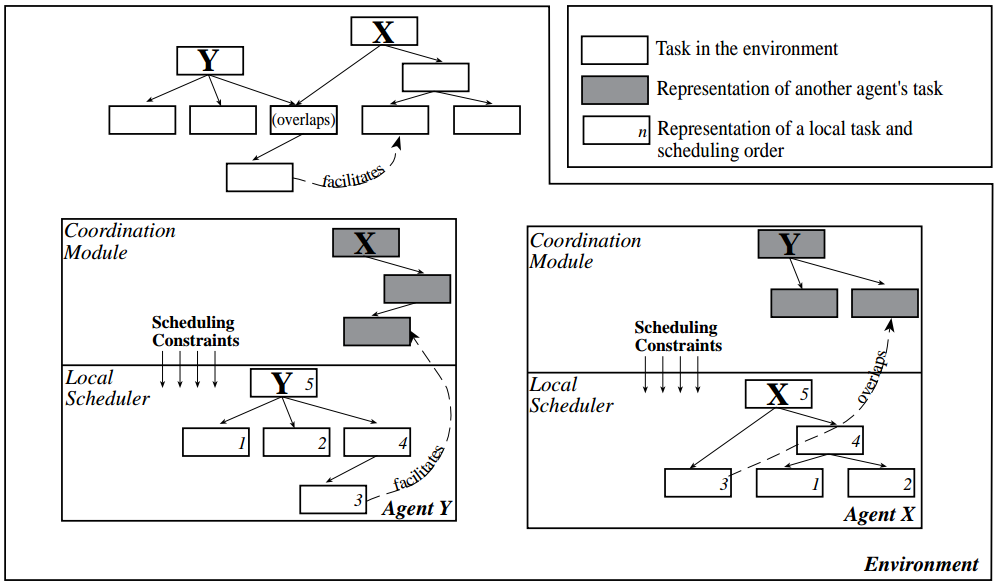
\includegraphics[scale=0.42]{figuras/pgp/pgp_generalized.png}
    \caption{Exemplo de estrutura GPGP. Fonte: \citeonline{decker1992generalizing}.}
    \label{fig:pgp_generalized}
\end{figure}

A estrutura do padrão GPGP pode ser exemplificada pela Figura \ref{fig:pgp_generalized}. Basicamente, a informação flui pelo ambiente através do mecanismo de coordenação do agente, \textit{Coordination Module}, e do mecanismo de agendamento local, \textit{Local Scheduler}. Primeiro, um determinado ambiente e/ou domínio de tarefa, em conjunto com um determinado agente, induz determinados relacionamentos de coordenação (\textit{RCs}) entre tarefas nesse ambiente \cite{decker1992generalizing}. 

Cada agente segue algum algoritmo de coordenação que detecta ou até mesmo hipotetiza \textit{RCs} e reage de acordo. Em seguida, este algoritmo produz certos comportamentos, por exemplo, (i) a criação e refinamento de restrições no agendamento local, e (ii) a negociação e criação de estruturas de dados internas \cite{decker1992generalizing}.

%Podemos relacionar como o comportamento do algoritmo de coordenação (criar e refinar restrições) afeta o comportamento do agendamento do agente baseando a análise em certas propriedades do mecanismo de agendamento local.

%O comportamento de escalonamento das tarefas do agente através do algoritmo GPGP afeta o desempenho do agente e de qualquer organização da qual ele faz parte, não apenas ao ordenar e executar tarefas, mas também ao incorrer em custos, como comunicação e tempo \cite{decker1992generalizing}.



\item[Modelagem:] Este padrão pode ser exemplificado pela Figura \ref{fig:pgp_generalized}. 
    
\item[Exemplo:] 

De modo a exemplificar uma utilização do padrão, é apresentado o caso abordado no artigo \textit{Coordinated Hospital Patient Scheduling} \cite{decker1998coordinated} e exemplificado pela Figura \ref{fig:gpgp_hospital_example}.




\begin{figure}[h!]
    \centering
    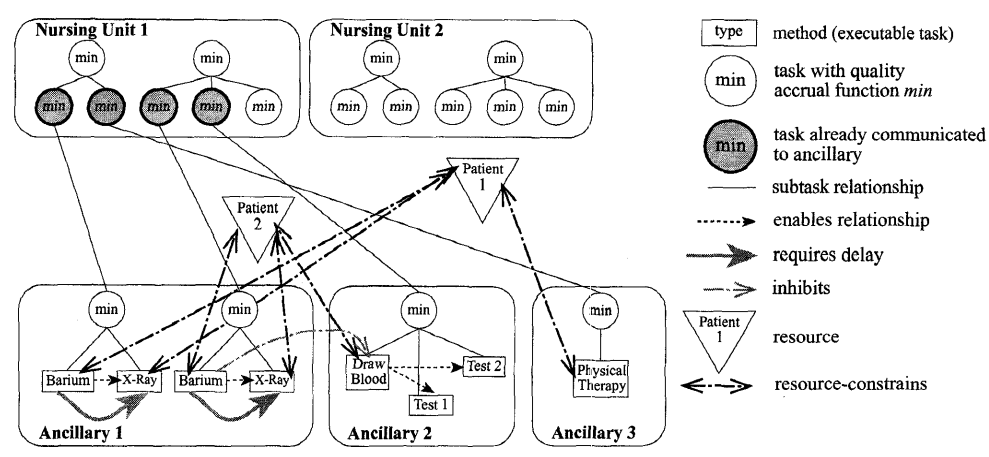
\includegraphics[scale=0.42]{figuras/pgp/gpgp_hospital_example.png}
    \caption{Exemplo de agendamento de um paciente. Fonte: \citeonline{decker1998coordinated}.}
    \label{fig:gpgp_hospital_example}
\end{figure}


Os pacientes de um hospital geral residem em unidades organizadas por ramos de medicina, como ortopedia ou neurocirurgia. Todos os dias, os médicos solicitam que determinados testes e/ou terapias sejam realizados como parte do diagnóstico e tratamento de um paciente. Os testes são realizados por departamentos auxiliares separados, independentes e dispostos em diferentes locais do hospital. O departamento de radiologia, por exemplo, presta serviços de raio-x e pode receber pedidos de várias unidades diferentes no hospital.

Além disso, cada teste pode interagir com outros testes em relacionamentos, tais como: autorizar, requisitar, atrasar, impedir outros testes. Essas relações entre tarefas indicam quando a execução de uma tarefa altera as características de outra tarefa e, neste caso, é principalmente a duração. A partir dessa visão da estrutura da tarefa, o problema de agendamento do hospital tem as seguintes características peculiares:
\begin{itemize}
    \item Tarefas não têm redundância. Cada teste só pode ser feito por um único departamento auxiliar;
    \item As funções de acúmulo de qualidade de tarefas não executáveis são sempre mínimas. Isto porque aqui todos os testes precisam ser feitos;
    \item A qualidade final não é importante: um teste é concluído ou não é, e
    \item Agentes diferentes, representando diferentes \textit{Nursing Units} (unidades de enfermagem) ou diferentes \textit{Ancillary Units} (unidades auxiliares), podem usar diferentes regras para fazer programações locais. Por exemplo, as \textit{Nursing Units} podem tentar minimizar o tempo de permanência do paciente, enquanto a \textit{Ancillary Unit}  tenta maximizar o uso do equipamento e/ou minimizar os tempos depreendidos em configuração dos mesmos.
\end{itemize}


Neste problema de agendamento do hospital, alguns testes só podem ser feitos com o paciente fisicamente presente. Assim, surge um problema de restrição de recursos, ou \textbf{\textit{shared resource-constrained relationship}}, em que \textbf{o paciente se torna um recurso crucial não-compartilhável} para diferentes agentes. 

Quando vários agentes tentam usar o mesmo recurso não compartilhável em horários sobrepostos, apenas um agente pode realmente obter o recurso e executar seu trabalho. Outros que não falharam em obter o recurso, desperdiçaram tempo e esforço da unidade.

A ideia por trás do mecanismo de coordenação com restrição de recursos é que quando um agente pretende executar uma tarefa com restrição de recurso, ele deve enviar um lance informando o intervalo de tempo que necessita do recurso e a sua prioridade local. 

Após um pequeno \textit{delay} de comunicação, ele passa a conhecer todos os lances que foram dados pelos outros agentes ao mesmo tempo que seu próprio lance. Como todos os agentes que fizeram lances terão as mesmas informações inicias, se todos usarem a mesma regra comumente aceita para decidir quem receberá o intervalo de tempo, eles poderão obter o mesmo resultado nessa rodada de lances.

O agente que ganhou manterá sua programação e executará essa tarefa no intervalo de tempo que ele solicitou no lance, e todos os outros marcarão esse intervalo de tempo com um compromisso de não fazer e ou sequer tentar executar a tarefa neste período que necessite do recurso. Todos os agentes que não obtiveram seus intervalos de tempo nessa rodada serão reprogramados e realizarão lances novamente. O processo detalhado é o seguinte:




Por exemplo, suponha que o atraso de comunicação seja uma unidade de tempo e que hajam três agentes e tarefas da seguinte maneira: 
\begin{itemize}
    \item O agente A tem as tarefas A11 e A12, cada uma de duração 3;
    \item O agente B tem a tarefa B11 de duração 2;
    \item O agente C tem a tarefa C11 de duração 4 e a tarefa C12 de duração 1;
    \item A11, B11 e C11 se caracterizam como \textbf{\textit{shared resource-constrained relationship}}.
\end{itemize}

O fluxo seria o seguinte:
\begin{description}
    \item [Tempo 0:] cada agente comunica estruturas de tarefas.
    \item [Tempo 1:] cada agente faz sua própria programação local: Agente A: A11 (1-3), A12 (4-6); Agente B: Bll (1-2); Agente C: C12 (1-1). Momentaneamente a tarefa C11 não está no calendário local do Agente C. A razão podem ser causas externas, como C11 não estar habilitado.
    
    O Agente A envia um lance para o intervalo de tempo 1-3 com prioridade 3.
    
    O agente B envia um lance para o intervalo de tempo 1-2 com prioridade 4.

    \item [Tempo 2:] cada agente reúne informações sobre o lance que aconteceu no tempo 1.

    O Agente A descobre que outro agente ganhou o intervalo de tempo de 1 a 2, por isso marca esse intervalo de tempo como ocupado e, em seguida, tenta se reprogramar. Seus novos horários são: A12 (2-4), A11 (5-7). 
    
    O Agente A envia um lance de 5-7 com prioridade 3.
    
    O Agente B ganhou, por isso mantém o seu horário e inicia a execução de B11.
    
    O Agente C coloca C11 (3-6) na programação geral. O Agente C envia um lance para 3-6 com prioridade 2.
    
    \item [Tempo 3:] o Agente A descobre que ganhou, por isso mantém sua programação e começa a executar A12.
    
    O Agente C descobre que perdeu, por isso marca o intervalo de tempo 5-7 ocupado. A nova programação é C11 (7-10). 
    
    O Agente C envia um lance para o intervalo de tempo 7-10.
    
    \item [Tempo 4:] o Agente C venceu, ele mantém sua programação e, portanto, aguardará até o tempo 7 para iniciar sua execução.
    
\end{description}

\item[Implementação:] a fim de demonstrar este padrão, o código apresentado no Apêndice \ref{appendix:gpgp} simula o fluxo do contexto apresentado acima.



\end{description}

\begin{comment}O GPGP é uma abordagem de coordenação independente de domínio, deste modo, é possível adotar alguma linguagem de representação que represente o conjunto atual de tarefas pretendidas do agente  \cite{decker1998coordinated}. Tal linguagem pode permitir:

\begin{itemize}
    \item A representação de estruturas de tarefas são hierarquias de abstração cujas folhas são ações básicas instanciadas ou “métodos executáveis”;
    \item A especificação de características que mudam dinamicamente e características de tarefa incertas que afetam as preferências de um agente para algum estado do mundo, incluindo tarefas com prazos rígidos ou flexíveis;
    \item Indicação dos relacionamentos entre tarefas locais ou não locais ou recursos que afetam as características de preferência do agente \cite{decker1998coordinated}.
\end{itemize}

Um agente que usa a abordagem GPGP fornece para o sistema um mecanismo para recuperar seus planos e um mecanismo de planejamento que tenta maximizar a utilidade de suas tarefas para o sistema como um todo \cite{decker1998coordinated}. Cada mecanismo GPGP examina as mudanças na estrutura de tarefas para determinadas situações. Em seguida, responde assumindo compromissos locais e não locais, possivelmente criando novas ações de comunicação para transmitir compromissos ou informações de estrutura de tarefas parciais para outros agentes \cite{decker1998coordinated}.

O conjunto de mecanismos de coordenação é extensível e tais mecanismos podem ser utilizados em conjunto em resposta a uma situação específica do ambiente. Inicialmente, \citeonline{decker1998coordinated} definiu cinco mecanismos de coordenação:

\begin{itemize}
    \item Atualização de pontos de vista não locais: cada agente detecta as possíveis relações de coordenação e em seguida comunica as estruturas de tarefas relacionadas;
    \item Comunicação dos resultados quando eles forem solicitados por outros mecanismos;
    \item Lidar com redundância simples: quando mais de um agente deseja executar um método redundante, um agente é escolhido aleatoriamente para executá-lo e enviar o resultado para os outros agentes interessados.
    \item Manipulação de relacionamentos rígidos: por exemplo, uma tarefa A que deve vir antes da tarefa B;  do lado predecessor. Neste relacionamento, há, portanto, a tarefa "predecessora" (A) e a tarefa "sucessora" B.
    \item Manipulação de relacionamentos flexíveis do lado predecessor: por exemplo, se a tarefa A for executada antes da tarefa B, a execução de B será talvez mais rápida ou retornará melhores resultados, mas não é estritamente necessária/obrigatória \cite{decker1998coordinated}.
\end{itemize}
\end{comment}

